\subsection {Metaheurísticas}  
El siguiente tema abordara sobre las metaheurísticas, sus características y principales ejemplos.
\subsubsection {Concepto de heurística}  
Según \cite{[ZANAEVA]} un heurístico es un “procedimiento simple, a menudo basado en el sentido común, que se supone que ofrecerá una buena solución (aunque no necesariamente la óptima) a problemas difíciles, de un modo fácil y rápido”. Las heurísticas se utilizan, por ejemplo, cuando no existe un método exacto de resolución, cuando existe un método exacto que consume mucho tiempo para ofrecer la solución óptima, cuando existen limitaciones de tiempo o como paso intermedio para obtener una solución inicial para la aplicación de otra técnica. Según \cite {[SILVER]} se propone la siguiente clasificación de métodos de resolución mediante heurísticas:
\begin{itemize}
\item \textbf{Métodos constructivos: } Se caracterizan por construir una solución definiendo diferentes partes de ella en sucesivos pasos.
\item \textbf{Métodos de descomposición: } Dividen el problema en varios más pequeños y la solución se obtiene a partir de la solución de cada uno de estos.
\item \textbf{Métodos de reducción: } Tratan de identificar alguna característica de la solución que permita simplificar el tratamiento del problema.
\item \textbf{Métodos de manipulación del modelo: } Obtienen una solución del problema original a partir de otra de otro problema simplificado (con menos restricciones, linealizando el problema, etc.)
\item \textbf{Métodos de búsqueda por entornos: } En las que se parte de una solución inicial a la que se realizan modificaciones en sucesivas iteraciones para obtener una solución final. En cada iteración existe un conjunto de soluciones vecinas candidatas a ser nueva solución en el proceso. En este grupo se encuadran las técnicas metaheurísticas.
\end{itemize}

\subsubsection {Características principales de las metaheurísticas} 

Las técnicas metaheurísticas son procedimientos de búsqueda que tampoco garantizan la obtención del óptimo del problema considerado y que también se basan en la aplicación de reglas relativamente sencillas.\\ 
\hspace*{1cm}A diferencia de las heurísticas, las técnicas metaheurísticas tratan de escapar de óptimos locales orientando la búsqueda en cada momento dependiendo de la evolución del proceso de búsqueda. \cite{[SADIQBIB]} dice que las metaheurísticas tienen como características:
\begin{itemize}
\item \textbf{Ser ciegas: } No saben si llegan a la solución óptima. Por lo tanto, se les debe indicar cuándo deben detenerse.
\item \textbf{Ser algoritmos de aproximación:} Por tanto no garantiza la obtención de la solución óptima.
\item \textbf{Aceptan ocasionalmente soluciones ineficientes: } Sin embargo pueden ser de utilidad para acceder a nuevas regiones y escapar de óptimos locales.
\item \textbf{Ser relativamente sencillos:} Todo lo que se necesita es una representación
adecuada del espacio de soluciones, una solución inicial (o un conjunto de ellas) y un mecanismo para explorar el campo de soluciones.
\item \textbf{Ser generales:} Prácticamente se pueden aplicar en la resolución de cualquier problema de optimización de carácter combinatorio. Sin embargo, la definición de la técnica será más o menos eficiente en la medida en que las operaciones tengan relación con el problema considerado.
\item \textbf{Ser impredecibles:} La regla de selección depende del instante del proceso y de la historia hasta ese momento. Si en dos iteraciones determinadas la solución es la misma, la nueva solución de la siguiente iteración no tiene por qué ser necesariamente la misma.
\end{itemize}

\hspace*{1cm}Aunque las soluciones que ofrecen los técnicas metaheurísticas no son las óptimas y, en general, ni siquiera es posible conocer la proximidad de las soluciones al óptimo, permiten estudiar problemas de gran complejidad de una manera sencilla y obtener soluciones suficientemente buenas en tiempos razonables.\\

De acuerdo a \cite{[BLUMROLI]} las metaheurísticas se pueden clasificar según:
\begin{itemize}
    \item Si están inspiradas en procesos naturales
    \item Si son dinámicas o estáticas
    \item Si manejan memoria
    \item Si están basados en poblaciones y manejan varias soluciones por proceso
    \item Si utilizan técnicas de agrupamiento 
\end{itemize}

\subsubsection {Algoritmo voraz (Greedy)}
Los algoritmos voraces (del inglés greedy) reciben esta denominación por las siguientes razones según \cite{[CORMENL]}:
\begin{itemize}
\item Siempre escoge el mejor candidato para formar parte de la solución: Aquel que tenga mejor valor de la función objetivo, lo que constituye el cumplimiento de cierto criterio goloso de selección.
\item Esta elección es única e inmodificable dado que no analiza más allá los efectos de haber seleccionado un elemento como parte de la solución. No deshacen una selección ya realizada: una vez incorporado un elemento a la solución permanece hasta el final y cada vez que un candidato es rechazado, lo es permanentemente.
\end{itemize}
\hspace*{1cm}Se sabe sin embargo la calidad de los algoritmos voraces está en relación con las características de las instancias que pretenden resolver: puede arrojar muy buenos resultados para determinadas instancias del problema pero para otras no. Otro inconveniente que presentan es que se estancan en óptimos locales de las funciones que pretenden optimizar y quizá no analizan vecindades más allá del criterio goloso por lo que pueden estar dejando de considerar al óptimo global.

A continuación el pseudocodigo \ref{lst:PseudocodigoGreedy} que muestra cómo funciona:
\begin{lstlisting}[language=C++, caption=Pseudocódigo base para el algoritmo greedy., label=lst:PseudocodigoGreedy]
/* Algoritmo de Greedy*/
Inicio
  S=Solucion Inicial
  Mientras (Condición establecida){
  S´= Se genera una solución nueva en base a la inicial
    if (S´> S){
        S = S´
    }
  }
  retorno S
Fin;
\end{lstlisting}

\hspace*{1cm}A diferencia de otros algoritmos éste no almacena soluciones adicionales y entre sus virtudes se encuentra en la simplicidad que tiene y por tanto, menor manejo de recursos, sin embargo su defecto se encuentra en el hecho de que no toma decisiones alejadas de la solución inicial, si ésta no cumple con su objetivo se deshace el cambio anterior y continua con el procedimiento hasta que cumpla con la condición establecida.\\

\subsubsection {Búsqueda local}  
Según \cite{[ADPEREZ]}, la idea básica de los algoritmos de búsqueda local es iniciar con una solución inicial ya sea generada aleatoriamente o hallada con algún otro algoritmo; una vez obtenida se realiza una transformación aleatoria de sus valores para mejorar la solución. Dicha transformación se repite hasta que ya no se pueda mejorar más la solución o bien, que cumpla con ciertas condiciones.\\
\hspace*{1cm}En la figura \ref{fig:EXPLOCAL.png} se puede ver un ejemplo de una gráfica formada por las ciudades $(v, x, y, z)$, analizando la ruta de la izquierda se puede crear una nueva ruta reemplazando dos caminos que comprenden los puntos $(x,y)$ y $(v,z)$ haciendo los caminos $(x,v)$ y $(y,z)$ produciendo un nuevo tour que es el que se puede apreciar a la derecha de la misma imagen.\\
%\hspace*{1cm}La vecindad de I consiste de todas aquellas soluciones que se obtienen haciendo el reemplazo de pares arcos.\\
%¿Cuántos vecinos tiene I si consiste de n ciudades vecinas?La respuesta viene siendo un problema del tipo O($N^2$) ya que cada ciudad tiene una probabilidad de 1 de 7 para conectarse con la ruta más óptima.\\

    \begin{figure}[hbtp]
        \centering
            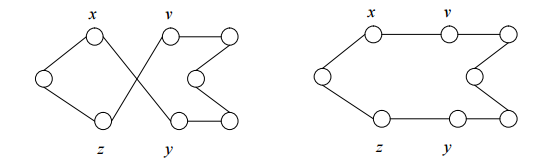
\includegraphics[width=0.6\textwidth]{MarcoTeorico/Imagenes/EXPLOCAL.png}
            \caption{Ejemplo de búsqueda local aplicado al TSP.}                       
            \label{fig:EXPLOCAL.png}
    \end{figure} 
    
\subsubsection {Recocido simulado}  

Recocido Simulado (SA por sus siglas en inglés) de acuerdo a \cite{[METROPOLIS]} es un método de optimización inspirado en el proceso de templado de metales. El algoritmo de recocido simulado es un método iterativo que inicia con una perturbación de cierto estado $s$. Mediante un proceso particular genera un estado vecino $s'$ al estado actual. Si la energía, o evaluación, del estado $s'$ es menor que la del estado $s$, se cambia el estado $s$ por $s'$. Si la evaluación de $s'$ es mayor que la de $s$ entonces se puede elegir $s'$ en lugar de $s$ con una cierta probabilidad que depende de las diferencias de las evaluaciones $\Delta f = f(s)-f(s') $ y de la temperatura actual del sistema $T$. La posibilidad de elegir un estado peor al actual es lo que le permite a SA salir de óptimos locales para poder llegar a los óptimos globales. La probabilidad de aceptar elegir un peor estado normalmente se calcula por la distribución de Boltzmann: $$ P(\Delta f, T) = e ^{\Delta f/T} $$
\hspace*{1cm}La cualidad de SA es que la temperatura va disminuyendo gradualmente conforme avanza la simulación. El código \ref{lst:recocidosimulado} representa una versión general del algoritmo de recocido simulado:\\

\begin{lstlisting}[language=HTML, caption=Pseudocódigo base para el algoritmo de recocido simulado., label=lst:recocidosimulado]
s := GeneraUnaSolucionInicial();
T := T0; g := 0;
mientras (CondicionesParoNoActivas(g, T)) hacer
    s' := Toma Un VecinoAleatorioDe(s);
    si ( f(s') < f(s))
        s := s';
    No
    //se usara la fórmula de temperatura
        si (Random(0, 1.0) < exp((f(s) - f(s'))/T)) 
            s := s';
        fin si;
    fin si;
g := g + 1; T := Actualiza(g, T);
fin mientras
\end{lstlisting}

%En la figura \ref{fig:RecocidoSimulado} se presenta un ejemplo propuesto de \cite{[GRANVILLE]}:  El problema consiste en disponer los píxeles en la imagen de tal manera que se minimice una función de energía potencial que causa que los colores similares se atraigan a distancias cortas y se repelan a distancias largas. En cada iteración se intercambian las posiciones de dos píxeles adyacentes. La imagen de la izquierda es obtenida con un protocolo de enfriado rápido, en el que la temperatura desciende rápidamente, y la de la derecha, con un protocolo lento, equiparables a los procesos de formación de sólidos amorfos y cristalinos respectivamente.

%    \begin{figure}[hbtp]
%        \centering
%            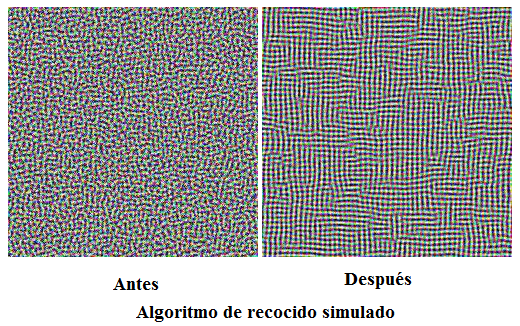
\includegraphics[width=0.6\textwidth]{MarcoTeorico/Imagenes/RecocidoSimulado.png}
%            \caption{Ejemplo de un problema de alineamiento de píxeles aplicando recocido simulado.}                       
%            \label{fig:RecocidoSimulado}
%    \end{figure} 


\subsubsection {Algoritmo genético}

Los algoritmos genéticos (AG) son métodos adaptativos que están basados en la teoría evolutiva de Darwin y la teoría genética de Mendel. En la naturaleza los individuos de una población compiten entre sí en la búsqueda de recursos tales como comida, agua y refugio. Incluso los miembros de una misma especie compiten a menudo en la búsqueda de un compañero. Aquellos individuos que tienen más éxito en sobrevivir y en atraer compañeros tienen mayor probabilidad de generar un gran número de descendientes.\\
\hspace*{1cm}Como se puede ver en la figura \ref{fig:agenetico} se tiene un grupo de individuos representado por círculos de colores, en algún momento 2 de estos círculos se juntarán y darán origen a un nuevo círculo, aunque posean algunas de las mismas características que sus padres es un ser único, este nuevo individuo se integrará al grupo y continuará su ciclo.

    \begin{figure}[hbtp]
        \centering
            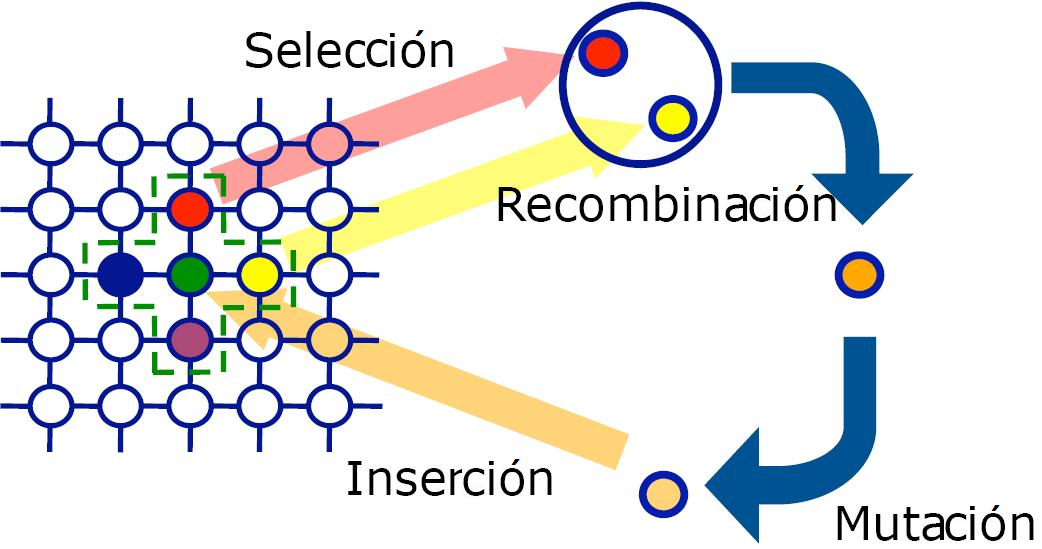
\includegraphics[width=0.7\textwidth]{MarcoTeorico/Imagenes/agenetico.png}
            \caption{Ejemplo de cómo funciona el algoritmo genético.}                       
            \label{fig:agenetico}
    \end{figure} 
    
\hspace*{1cm}A continuación se presentará un resumen basado en la idea general del algoritmo genético según \cite{[HOLLAND]}, \cite{[REEVES]}, \cite{[MICHALEWICZ]}, \cite{[DAVIS]},  \cite{[GOLDBERG]}. Las soluciones del problema se representan como un conjunto de parámetros llamados genes, los cuales agrupados forman un grupo de valores llamado cromosoma; el alfabeto que se usa para tratar con estos problemas puede ser cualquiera, pero para la siguiente explicación se usará el 1 y el 0. El conjunto de parámetros representando un cromosoma en específico se denomina fenotipo, el fenotipo contiene la información requerida para construir una solución el cual se refiere como genotipo.\\
\hspace*{1cm}La función de adaptación debe ser diseñada para cada problema de manera específica. Dado un cromosoma particular, la función de adaptación le asigna un valor numérico que se supone refleja el nivel de adaptación al problema del individuo representado por el cromosoma. Durante la fase reproductiva se seleccionan los individuos de la población para cruzarse y producir descendientes que constituirán, una vez mutados, la siguiente generación de individuos. La selección de padres se efectúa al azar usando un procedimiento que favorezca a los individuos mejor adaptados, ya que a cada individuo se le asigna una probabilidad de ser seleccionado que es proporcional a su función de adaptación. Es decir, los individuos bien adaptados se escogerán probablemente varias veces por generación, mientras que los pobremente adaptados al problema no se escogerán más que de vez en cuando. Una vez seleccionados los 2 padres, sus cromosomas se combinan utilizando habitualmente los operadores de cruce y mutación. Las formas básicas de dichos operadores se describen a continuación: 

\begin{itemize}
    \item El operador de cruce toma a los 2 padres seleccionados y divide sus genes en una posición escogida al azar para producir dos pares de cromosomas cada uno. Después se intercambian los cromosomas finales para crear una solución nueva (Figura \ref{fig:Codigo-genetico1}). Ambos descendientes heredan genes de cada uno de los padres. Este operador se conoce como operador de cruce basado en un punto.
    \item El operador de mutación se aplica a cada hijo de manera individual y consiste en la alteración aleatoria (normalmente con probabilidad pequeña) de cada gen componente del cromosoma.
\end{itemize}

\begin{figure}[hbtp]
    \centering
        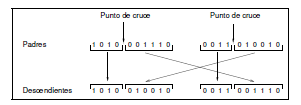
\includegraphics[width=0.7\textwidth]{MarcoTeorico/Imagenes/Codigo-genetico1.png}
        \caption{Operador de cruce basado en un punto.}                       
        \label{fig:Codigo-genetico1}
\end{figure} 
 
\hspace*{1cm}La figura \ref{fig:Codigo-genetico2} muestra la mutación del quinto gen del cromosoma.  Aunque el operador de cruce es más importante que el operador de mutación por proporcionar una exploración rápida del espacio de búsqueda, el operador de mutación asegura que ningún punto del espacio de búsqueda tenga probabilidad cero de ser examinado y es importante para asegurar la convergencia de un AG.

   \begin{figure}[hbtp]
        \centering
            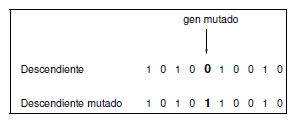
\includegraphics[width=0.7\textwidth]{MarcoTeorico/Imagenes/Codigo-genetico2.png}
            \caption{Operador de mutación.}                       
            \label{fig:Codigo-genetico2}
    \end{figure} 
    
\hspace*{1cm}El código \ref{lst:AlgoritmoGenetico} representa una versión general del algoritmo genético:\\

\begin{lstlisting}[language=C++, caption=Pseudocódigo base para el algoritmo algoritmo genético., label=lst:AlgoritmoGenetico]
/* Algoritmo Genético Simple */
Generar una población inicial().
Computar la función de evaluación de cada individuo().
MIENTRAS(NOT Terminado){
    /* Producir nueva generación */
    Ciclo (Tamaño población/2){
     /*Ciclo Reproductivo */
        1.-Seleccionar dos individuos de la anterior generación para el cruce (probabilidad de selección proporcional a la función de evaluación del individuo);
        2.-Cruzar con cierta probabilidad los dos individuos obteniendo dos descendientes;
        3.-Mutar los dos descendientes con cierta probabilidad. Computar la función de evaluación de los dos descendientes mutados;
        4.-Insertar los dos descendientes mutados en la nueva generación;
    }
}
SI( la población ha convergido) {
    Terminado := TRUE
}
Fin;

\end{lstlisting}
